\subsection{Proof Of Concept}\label{subsec:poc}

Um sicherzustellen, dass die Anforderungen an das System mit den gewählten Technologien umgesetzt werden können, wird zunächst ein Proof Of Concept implementiert.
Dieser Proof Of Concept hat einen deutlich kleineren Funktionsumfang als das Endprodukt.
Im Wesentlichen muss der Proof Of Concept beweisen, dass es möglich ist mit den gewählten Technologien Benachrichtigungen zu Versenden und zu empfangen.

\subsubsection{Funktionale Anforderungen}

Um dies zu ermöglichen werden die folgenden Features in eingeschränktem Umfang umgesetzt.

\textbf{F01 - Benachrichtigungen Versenden}

Mit dem Proof Of Concept muss es möglich sein, Benachrichtigungen von einem Client zu versenden.
Dementsprechend wird das Szenario "Benachrichtigung versenden" mit den folgenden Einschränkungen umgesetzt:

\begin{itemize}
    \item Es erfolgt kein Login und keine Authentifizierung.
    \item Es gibt nur einen vordefinierten Button.
    \item Es wird immer dieselbe vordefinierte Benachrichtigung versendet.
    \item Es werden keine Empfänger konfiguriert, die Benachrichtigung wird zurück an den Absender versendet.
\end{itemize}


\textbf{F02 - Benachrichtigungen empfangen}

Mit dem Proof Of Concept muss es möglich sein, Benachrichtigungen mit einem Client zu empfangen.
Dementsprechend wird das Szenario "Benachrichtigung empfangen" mit den folgenden Einschränkungen umgesetzt:

\begin{itemize}
    \item Es wird keine Liste von Benachrichtigungen geführt.
    \item Die Benachrichtigung wird in einem einfachen Textfeld im Mobile Client angezeigt.
\end{itemize}


\textbf{F04 - Über Benachrichtigungen Notifizieren}

Mit dem Proof Of Concept muss es möglich sein, über den Einfang von Benachrichtigungen notifiziert zu werden.
Dementsprechend werden die Szenarien "Foreground" und "Background" mit den folgenden Einschränkungen umgesetzt:

\begin{itemize}
    \item Die Notifizierung erfolgt ohne Audio Signal.
\end{itemize}

\clearpage
\subsubsection{Technische Anforderungen}

Damit der Proof Of Concept aussagekräftig ist, müssen die folgenden technischen Anforderungen umgesetzt werden:

\textbf{T01 - IPad Client}

Der für den Proof Of Concept umgesetzte Client muss auf einem IPad funktionieren und alle Anforderungen die an den
Proof Of Concept gestellt werden erfüllen. Kommunikation mit Cloud Service muss funktionieren. Kommunikation mit Messaging Service muss funktionieren.


\textbf{T04 - AWS Platform}

Der Cloud Service muss auf AWS deployed werden. Die Kommunikation zwischen Mobile Client und Cloud Service muss funktionieren.
Die Kommunikation mit Messaging Service muss funktionieren.


\subsubsection{Laufzeitsicht}

Im Wesentlichen muss der Proof Of Concept beweisen, dass es möglich ist mit den gewählten Technologien Benachrichtigungen zu Versenden und zu Empfangen.

Der Benutzer muss den Mobile Client auf dem IPad öffnen können. Aus dem Mobile Client muss der Benutzer über einen Butten eine Benachrichtigung versenden können.
Das Versenden dieser Benachrichtigung erfolgt an den Cloud Service.
Im Rahmen des Proof Of Concept wird eine Benachrichtigung immer an den Sender zurückgesendet. Dabei ist aber wichtig, dass die Benachrichtigung nicht direkt als
Antwort auf die Versenden-Anfrage geschickt wird. Stattdessen muss das Versenden der Benachrichtigung aus dem Cloud Service über den Message Service erfolgen. .

\begin{figure}[h]
    \centering
    \begin{minipage}[b]{1.0\textwidth}
        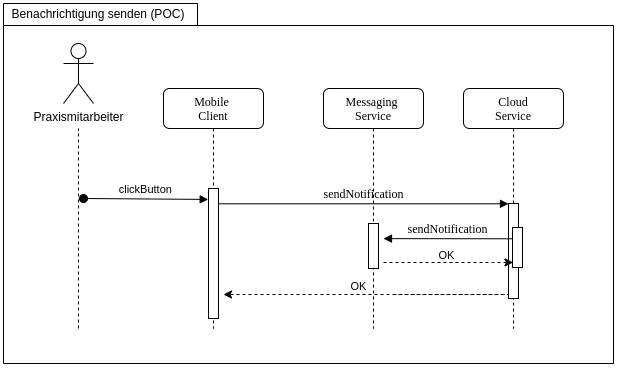
\includegraphics[width=\textwidth]{graphics/Sequence_POC_Send}
        \caption{Proof Of Concept - Benachrichtigung versenden}
    \end{minipage}
\end{figure}

\clearpage


Wurde eine Benachrichtigung über den Message Service an den Mobile Client versendet, muss diese vom Mobile Client empfangen werden.
Als Reaktion auf den Empfang der Benachrichtigung, muss der Inhalt der Benachrichtigung im Mobile Client angezeigt werden. Zudem
muss eine Push Benachrichtigung auf dem Host Gerät erfolgen.

\begin{figure}[h]
    \centering
    \begin{minipage}[b]{1.0\textwidth}
        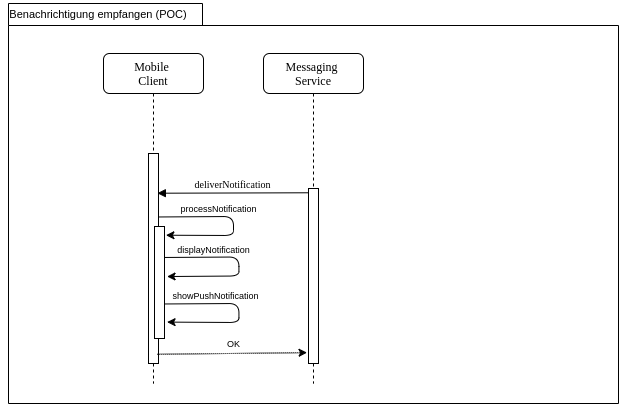
\includegraphics[width=\textwidth]{graphics/Sequence_POC_Receive}
        \caption{Proof Of Concept - Benachrichtigung empfangen}
    \end{minipage}
\end{figure}

\clearpage
